% !TeX spellcheck = en_US

\chapter{Introduction}

	Everyone of us already had to deal with a defective product. Years ago there was a good chance you could repair it on your own. But with electronics getting more complex and integrated into nearly everything we own, this is becoming impossible.
	
	One of the best examples are laptops. They originated from a - by design - highly modular hardware system. Every part has a standardized connector that makes it possible to build up a computer out of components from various manufacturers. But due to market demand the devices had to shrink more and more. To cope with the hassle of little space, manufactures began to integrate these single components in one another. This greatly reduces the overall product size.
	
	\begin{figure}[H]
		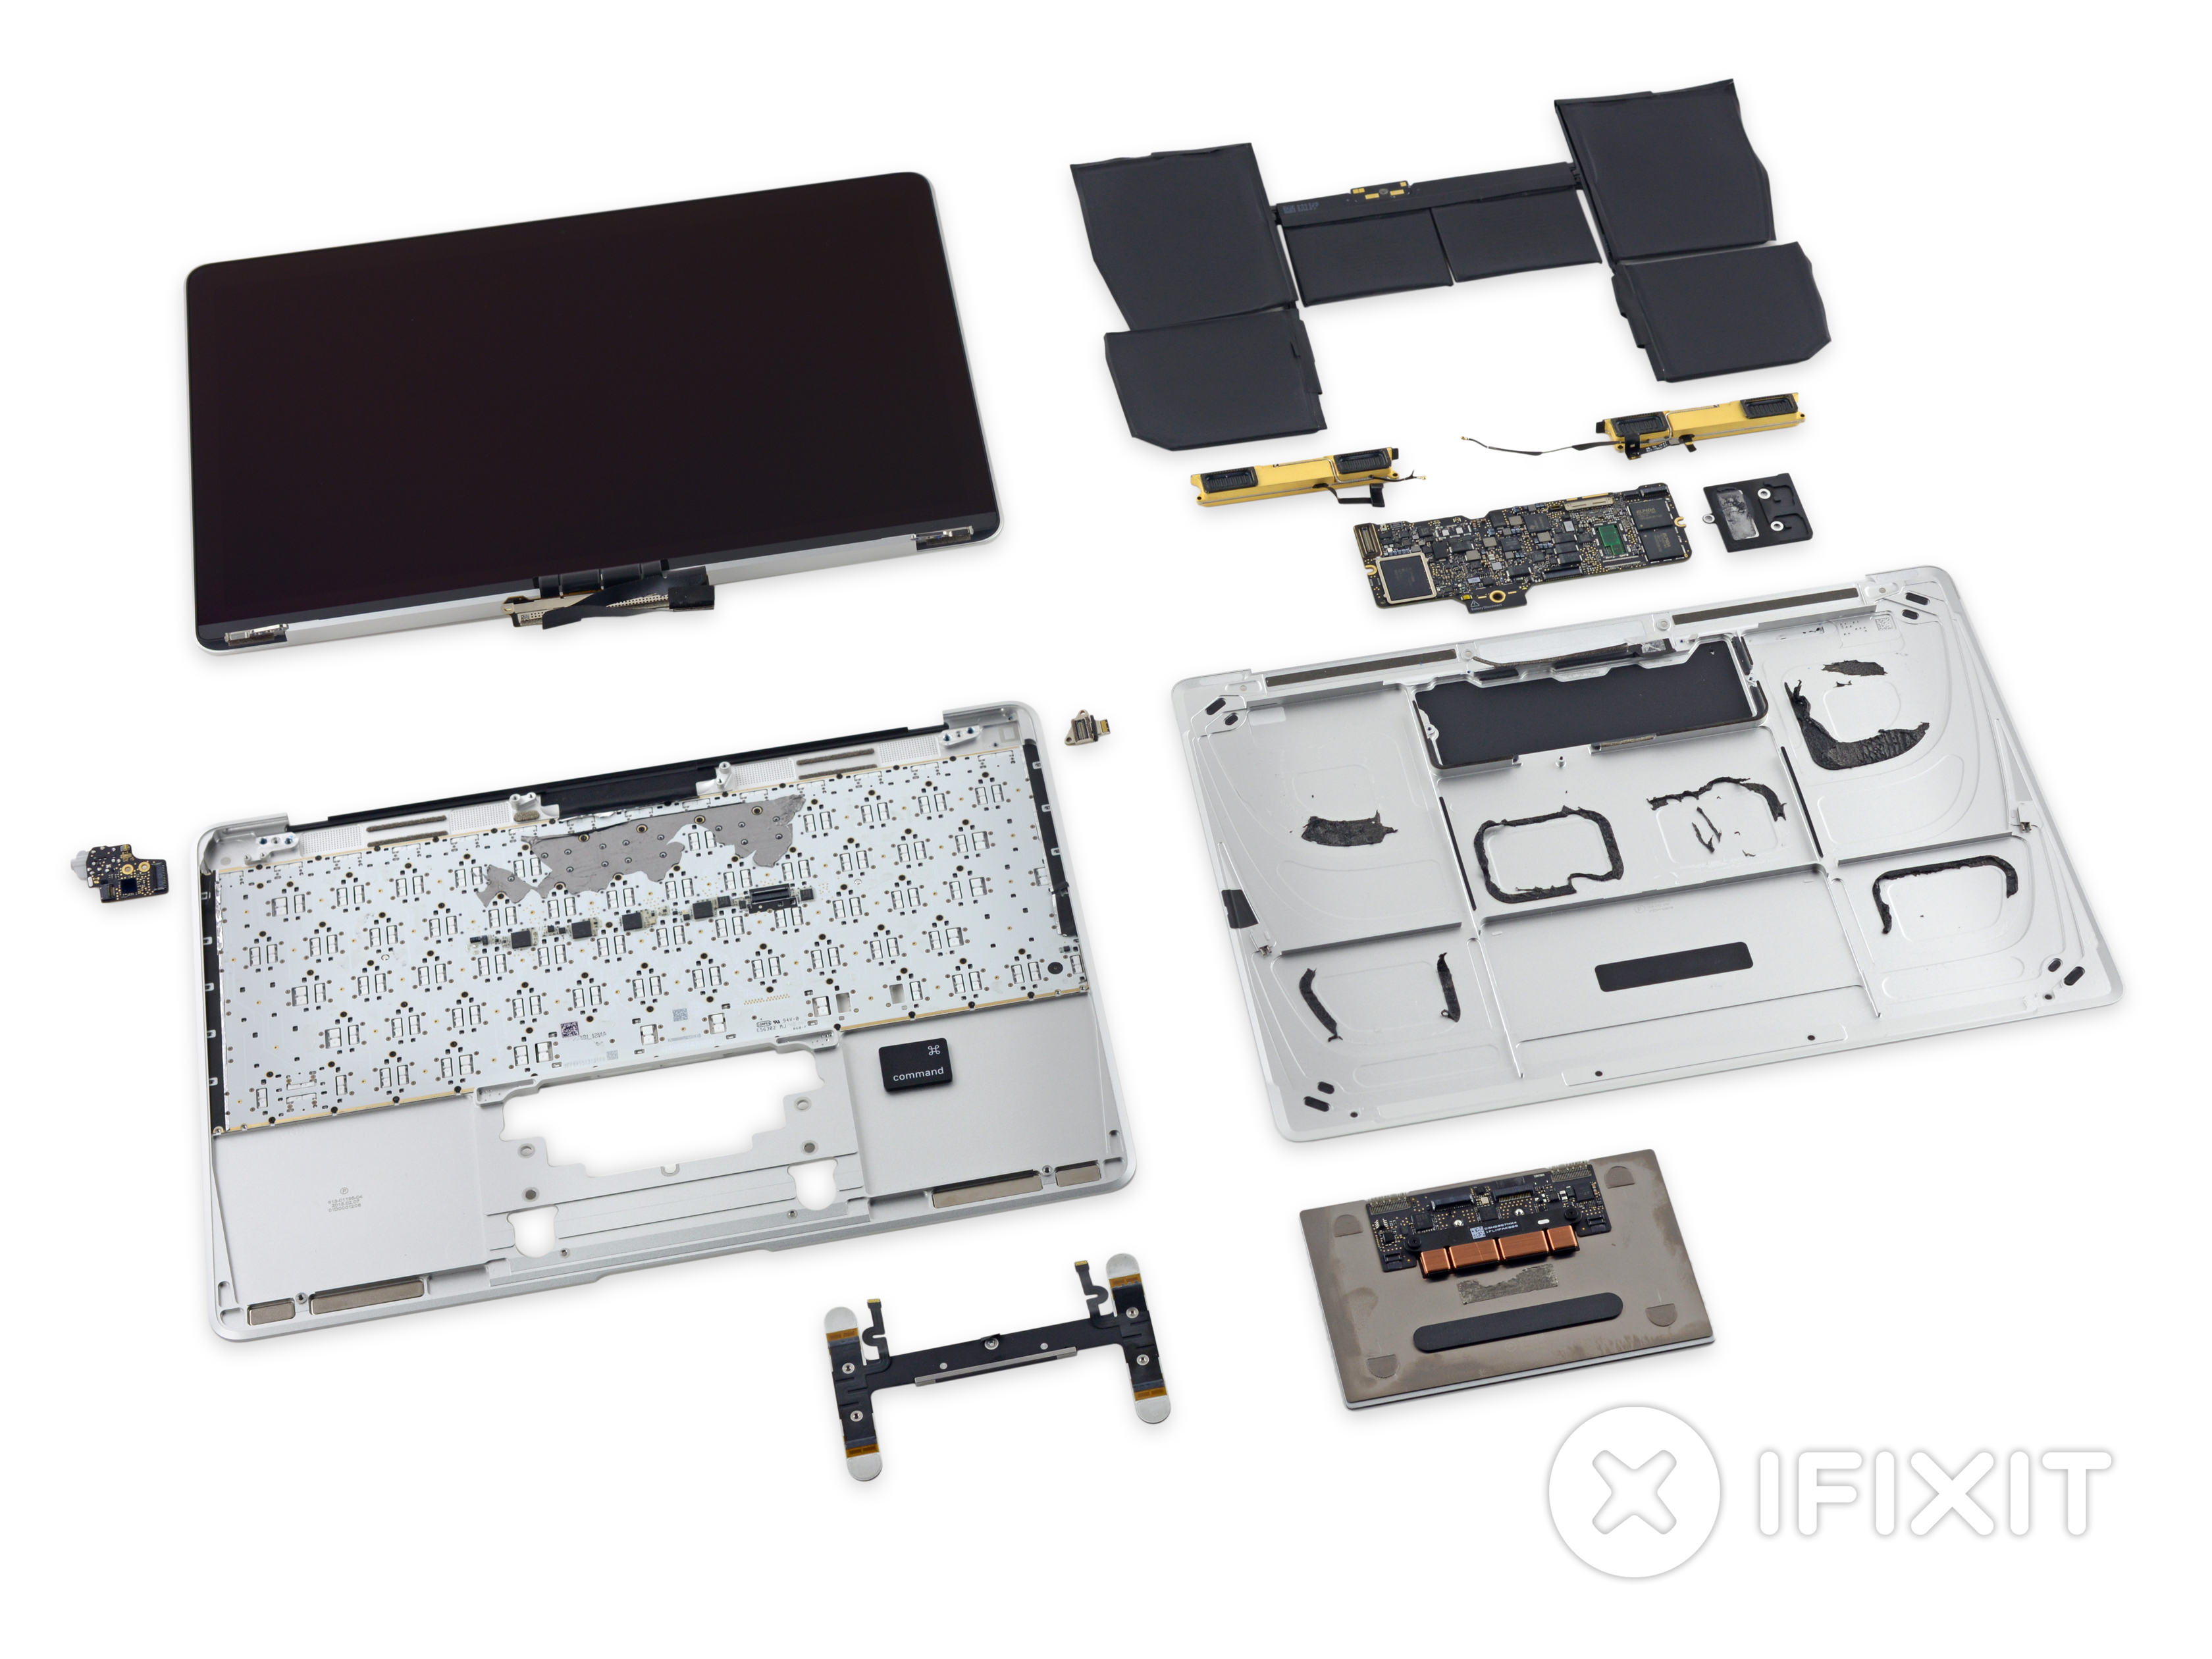
\includegraphics[width=\textwidth, trim=0 0 0 3cm, clip]{../images/ifixit-macbook-parts.jpg}
		\centering
		\caption[Disassembled Apple MacBook 2015 that got an iFixit Repairability Score of 1 out of 10]{Disassembled Apple MacBook 2015 that got a iFixit Repairability Score of 1 out of 10\footnotemark}
		\label{fig:ifixit-macbook-parts}
	\end{figure}
	\footnotetext{\url{https://de.ifixit.com/Teardown/Retina+MacBook+2015+Teardown/39841}}
	
	The most recent achievement of this approach can be seen in \autoref{fig:ifixit-macbook-parts}. The Apple MacBook 2015 is extremely thin, which led to reducing the size of the elctronics. Contradicting the traditional modular idea, everything from CPU to flash memory is soldered onto one single circuit board. It can only be replaced as one expensive part, if this is possible at all. The use of special adhesive saves the space needed for screws, yet it is not possible to handle for an end user.
	
	Of course this is problem not limited to mobile computer hardware. In almost every industry products become less and less fixable. Where 30 years ago one could repair your car by replacing the broken piece in a straightforward way, nowadays you do not even know what is defective without the help of a professional.
	
	\begin{figure}[H]
		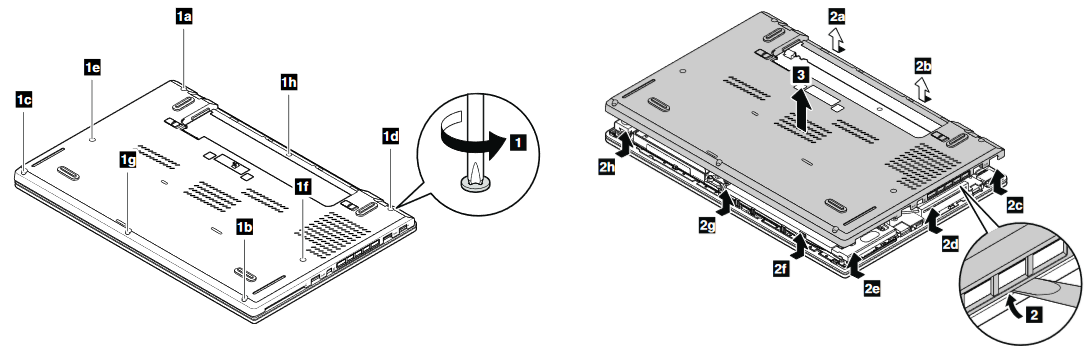
\includegraphics[width=\textwidth]{../images/common-manual.png}
		\centering
		\caption[Typical step-by-step manual for business laptop hardware, taken from Hardware Maintainance Manual by Lenovo Thinkpad]{Typical step-by-step manual for business laptop hardware, taken from Hardware Maintainance Manual by Lenovo Thinkpad\footnotemark}
		\label{fig:lenovo-hardware-manual}
	\end{figure}
	\footnotetext{\url{https://download.lenovo.com/ibmdl/pub/pc/pccbbs/mobiles_pdf/t440s_hmm_en_sp40a25360_04.pdf}}
	
	Furthermore the manufacturers do not want you to refurbish a product. They want you as the end user to buy new things.
	
	Solely the business sector demands products that are serviceable. \autoref{fig:lenovo-hardware-manual} shows an excerpt from a hardware maintenance manual for a professional business notebook by Lenovo. Almost all parts of this laptop are replaceable when following the instructions. But creating this manual, providing spare parts for end users and most importantly designing the product in a way it can be easily fixed is pretty expensive. This effort will be omitted with consumer products.
	
	\myparagraph{So what can you do?}
	
	For one thing, ask the manufacturer. In most cases a service option is available but can be really expensive. If these costs exceed the cost of a rebuy, you get a constructive total write-off. This happens quite fast considering costs for spare parts, shipping and time for the professional personal. When doing the repairs by yourself, you can save on the last two, which often are the major part of the expenses.
	
	But repairing stuff all by yourself is complicated, if one is not specially trained. Therefore there are manuals. Sometimes the manufactures provide these (see \autoref{fig:lenovo-hardware-manual}), but very often it is not in theirs financial interest to do so. Over the last years online communities and portals formed themselves to share and improve simple self-made manuals for repairing equipment.
	
	\begin{figure}[H]
		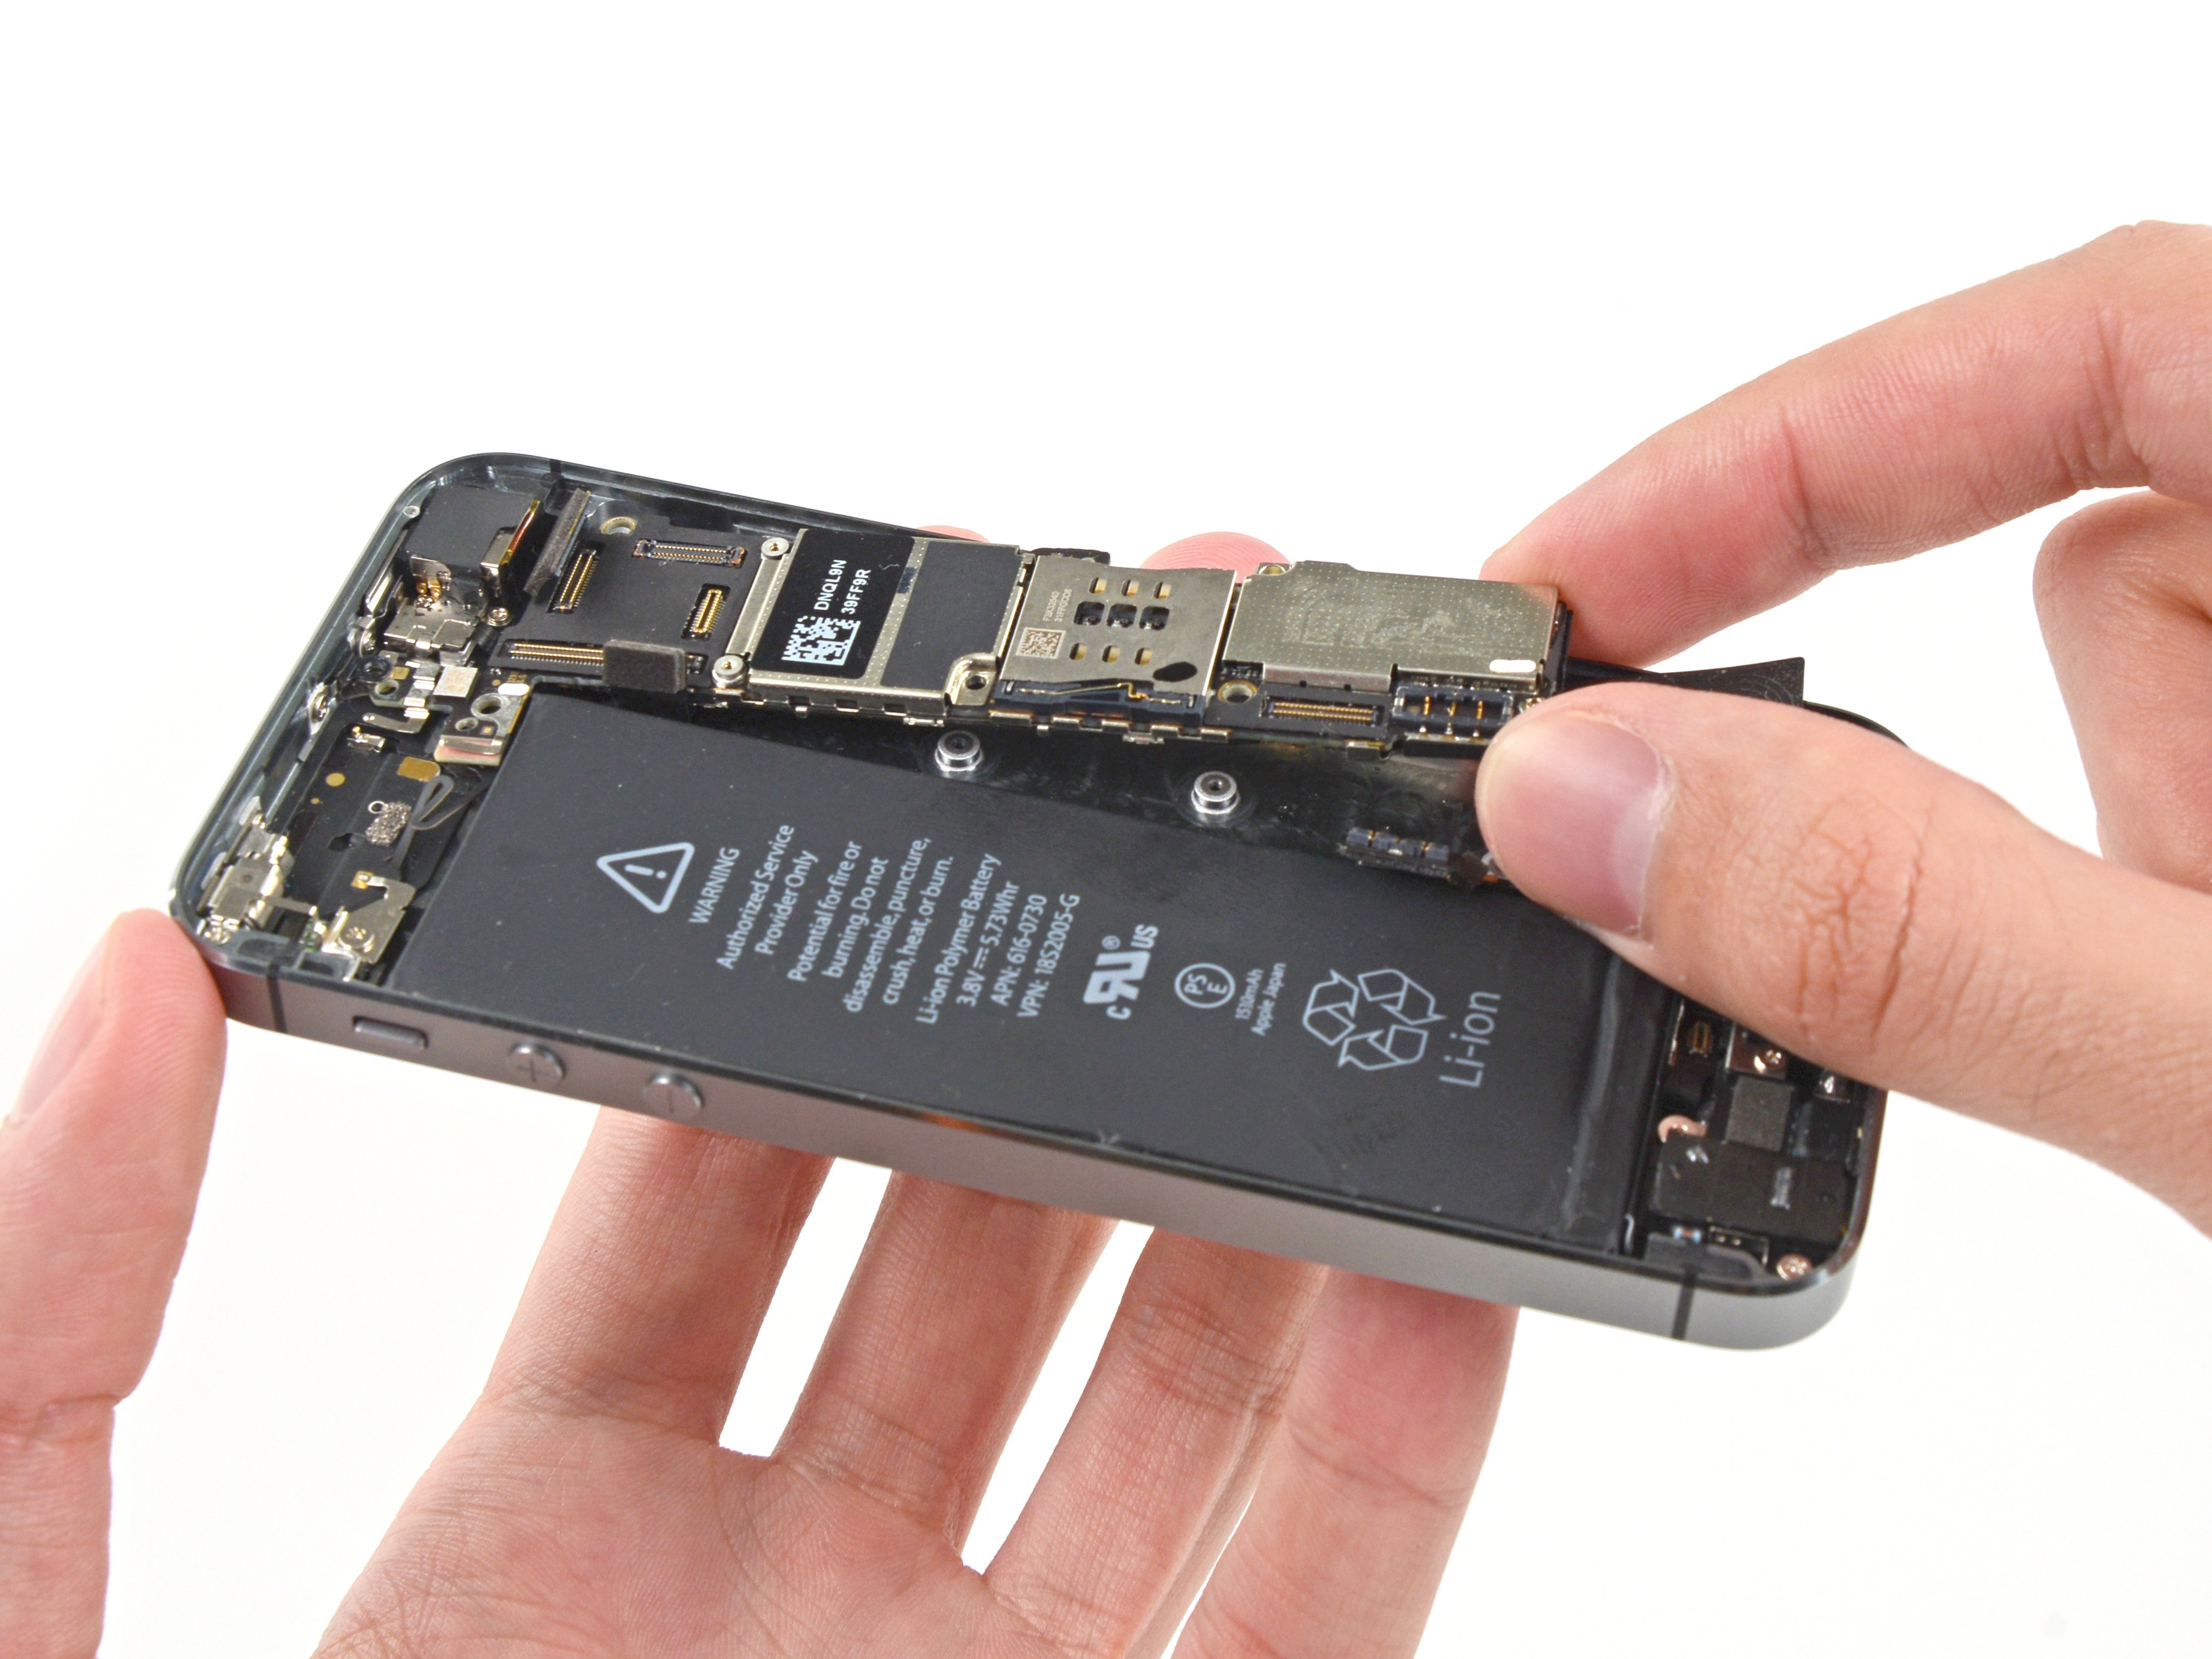
\includegraphics[width=0.8\textwidth]{../images/ifixit-iphone-logicboard.jpg}
		\centering
		\caption[Single step taken from an iFixit repair manual for replacing the Apple iPhone 5 logic board]{Single step taken from an iFixit repair manual for replacing the Apple iPhone 5 logic board\footnotemark}
		\label{fig:ifixit-iphone-logicboard}
	\end{figure}
	\footnotetext{\url{https://de.ifixit.com/Guide/id/20246}}
	
	One of these is iFixit, a US company with a website providing high quality step-by-step repair instructions. They mainly focus on electronic equipment like smartphones or notebooks. \autoref{fig:ifixit-iphone-logicboard} shows a picture that illustrates one step during the replacement of a circuit board inside a Apple iPhone 5. Additionally iFixit conveniently provides an online shop for all tools you might need to do your low-cost repair.
	
	uFixit improves the overall experience by adding augmented reality to the equation. Up till now, one has to find the correct manual on the internet and follow a step-by-step instruction set on some sort of second device. This is unhandy and the success of this operation greatly depends on the quality of the tutorial. Whereas iFixit instructions and photos are top-notch, much user-created content lacks clarity and professionalism.
	
	With uFixit however, we want to change that. All you need is a augmented reality device. It will recognize your broken product, find the corresponding tutorial and immediately start with instructions for repairing. Of course someone already tried this. One solution can be seen in \autoref{fig:bosch-flex-inspect}. A software helps engine service personal to visualize and highlight single components inside a car. It also proposes the best methods for replacing it with detailed descriptions.
	
	\begin{figure}[H]
		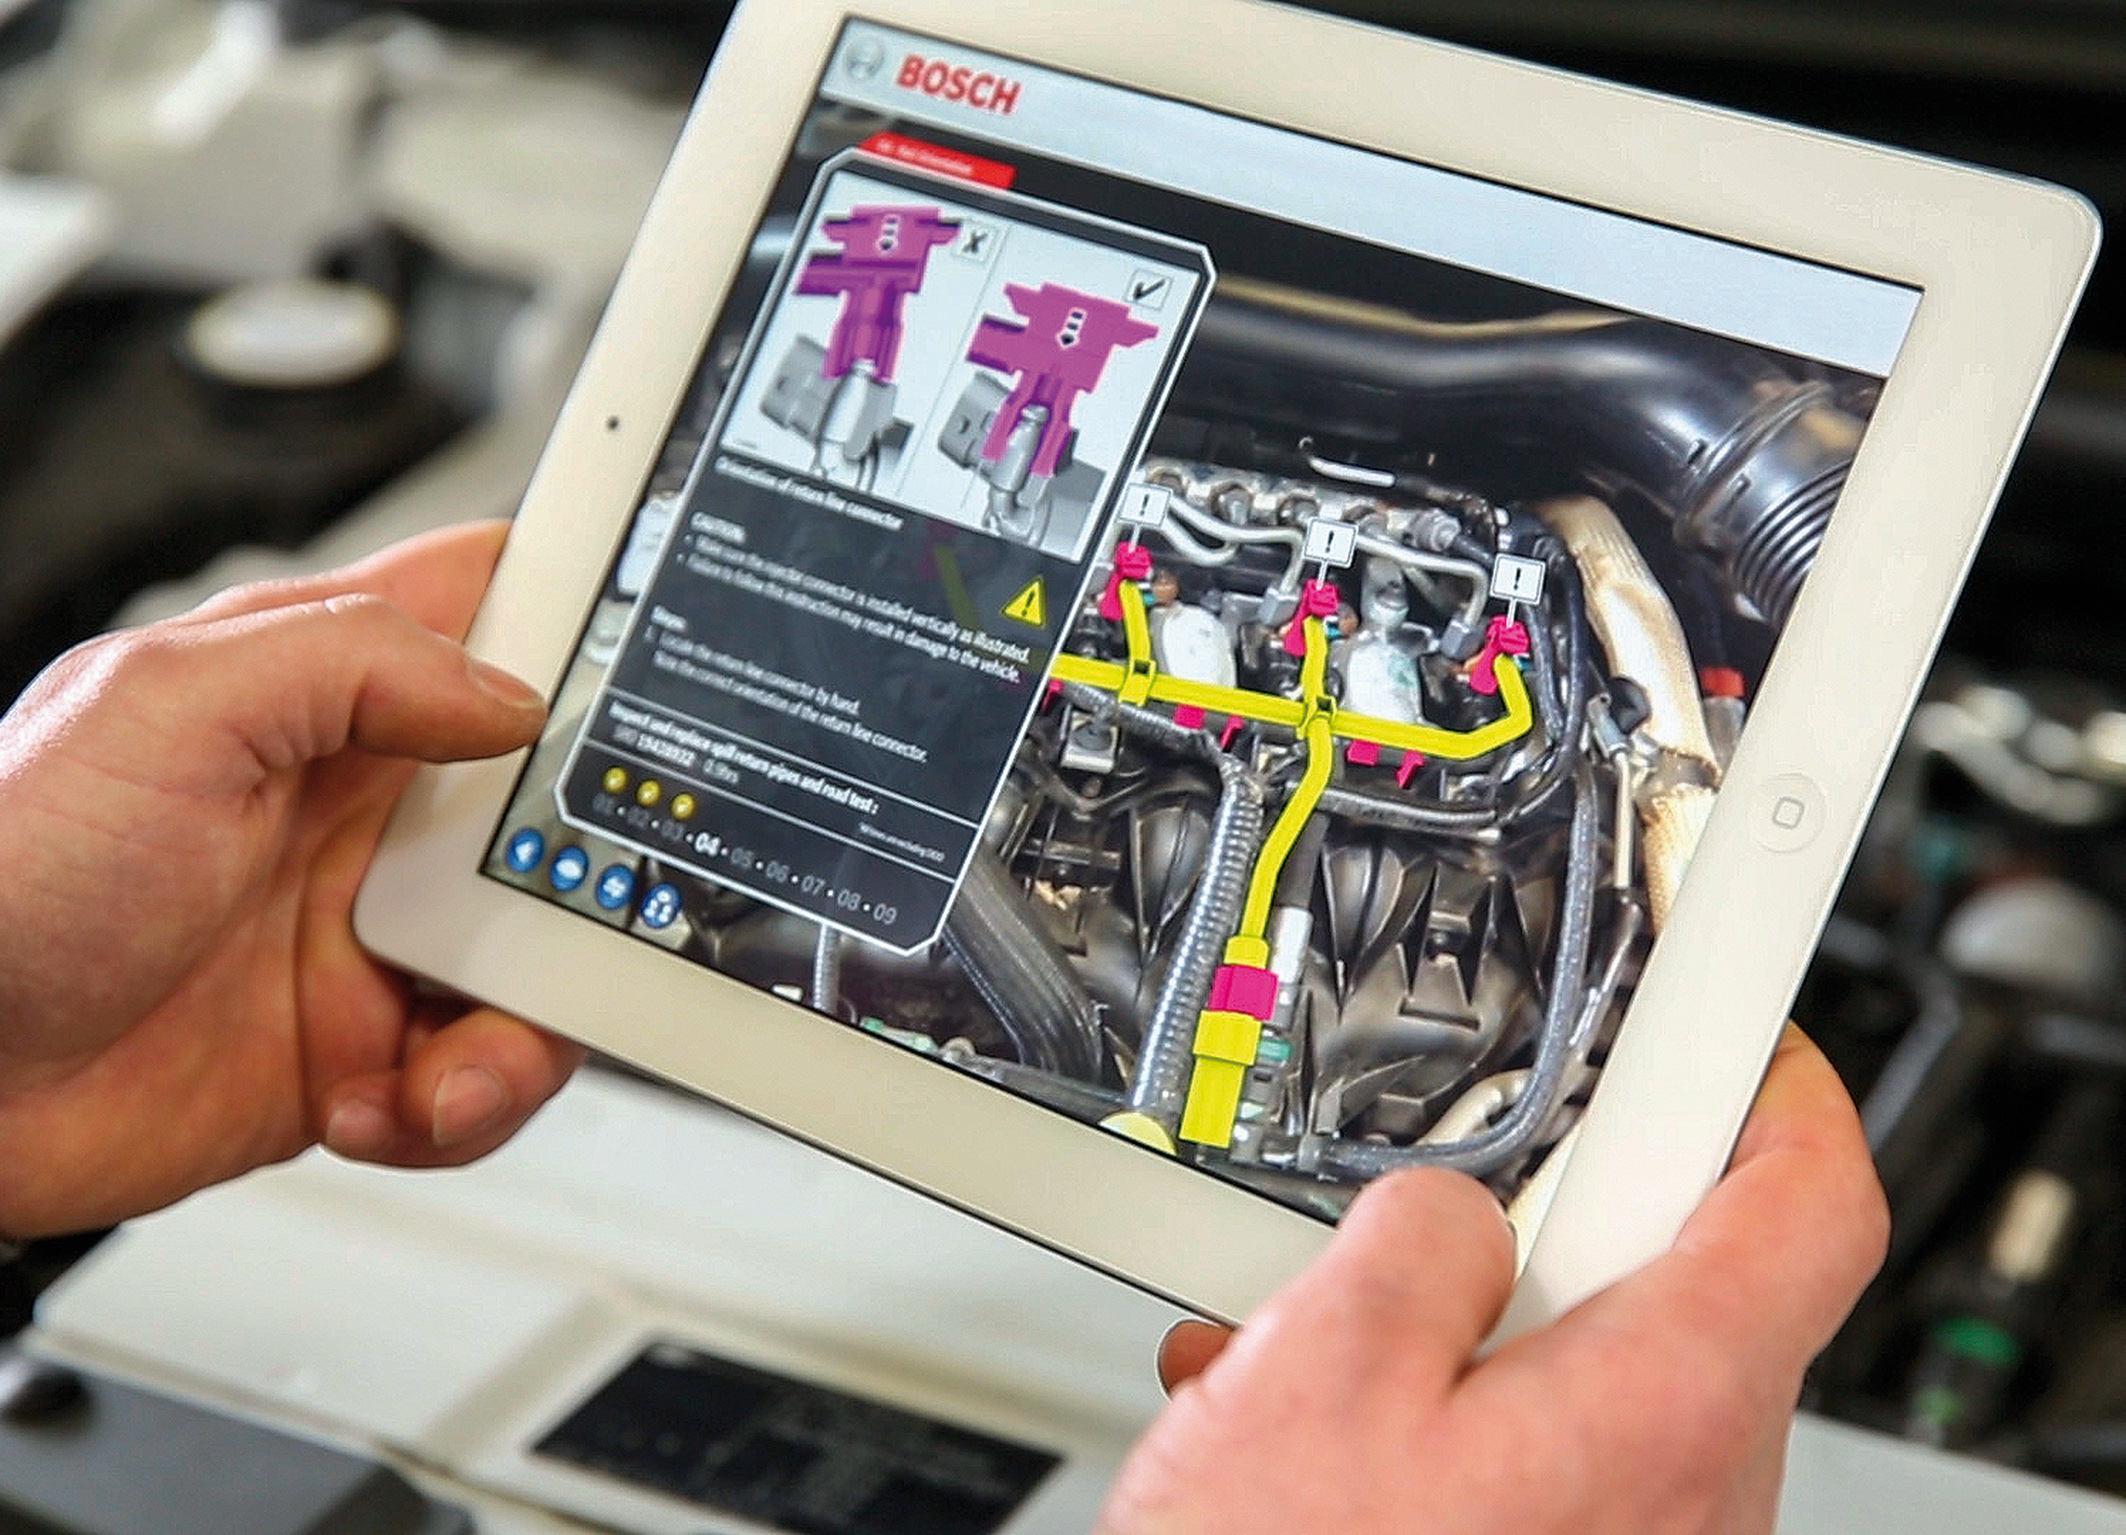
\includegraphics[width=0.9\textwidth]{../images/bosch-flex-inspect.jpg}
		\centering
		\caption[Professional augmented reality equipment by Bosch designed to help the repair shop personal]{Professional augmented reality equipment by Bosch designed to help the repair shop personal\footnotemark}
		\label{fig:bosch-flex-inspect}
	\end{figure}
	\footnotetext{\url{http://www.bosch-presse.de/presseforum/details.htm?txtID=6938&tk_id=109}}
	
	he drawback is that every single bit of content has to be created by professional 3D CAD engineers. It is nearly impossible to build a community in which everybody can design tutorial on their own.
	
	uFixit will solve this. Chapter 2 describes in detail how that works. Chapter 3 takes a look at the specific problems that have to be considered when using augmented reality. Finally chapter 4 presents a business plan for our solution.

